\documentclass[paper=a4, fontsize=11pt]{article}
\usepackage[utf8]{inputenc}
\usepackage[english,magyar]{babel}
\usepackage{amsmath}
\usepackage{graphicx} 
\usepackage{float}
\usepackage{rotating}
\usepackage{latexsym}
\usepackage{listings}

\addtolength{\oddsidemargin}{-.875in}
\addtolength{\evensidemargin}{-.875in}
\addtolength{\textwidth}{1.95in}
\addtolength{\topmargin}{-.9in}
\addtolength{\textheight}{1.6in}

\begin{document}
\begingroup
	\centering
	\LARGE Hálozatok\\
\vspace{1 cm}
\large Nagy Péter\\
\large M07ILF\\
\vfill
\large 2018.04.23.\\

\newpage

\tableofcontents
\newpage

\section{Bevezetés}
A beadandóban hálozatok szimulációját valosítottam meg. A felhasznált forrás kódokat.txt kiterjesztésű file-okban mellékeltem, valamint az adatsorokat és a mellék számításokat egy excell file-ban csatolom a jegyzőkönyv mellé.
\newpage

\section{Véletlen rekurzív fa}
A feladat az volt, hogy szimuláljunk egy véletlen rekurzív fát. Egy lépésben létrehozunk egy csúcsot adunk a hálozathoz és egyenlő valószinűséggel hozzácsatoljuk egy meglévő csúcshoz. 


\subsection{Fokszámeloszlás}
A szimulációban 100 db csúcsot hoztam létre. A fokszám eloszlásokat a következő képpen határozzuk meg:
\begin{align}
P_k=\frac{N_k}{N}
\end{align}
Ahol $N_k$ az adott csúcs fokszáma és N a csúcsok száma.
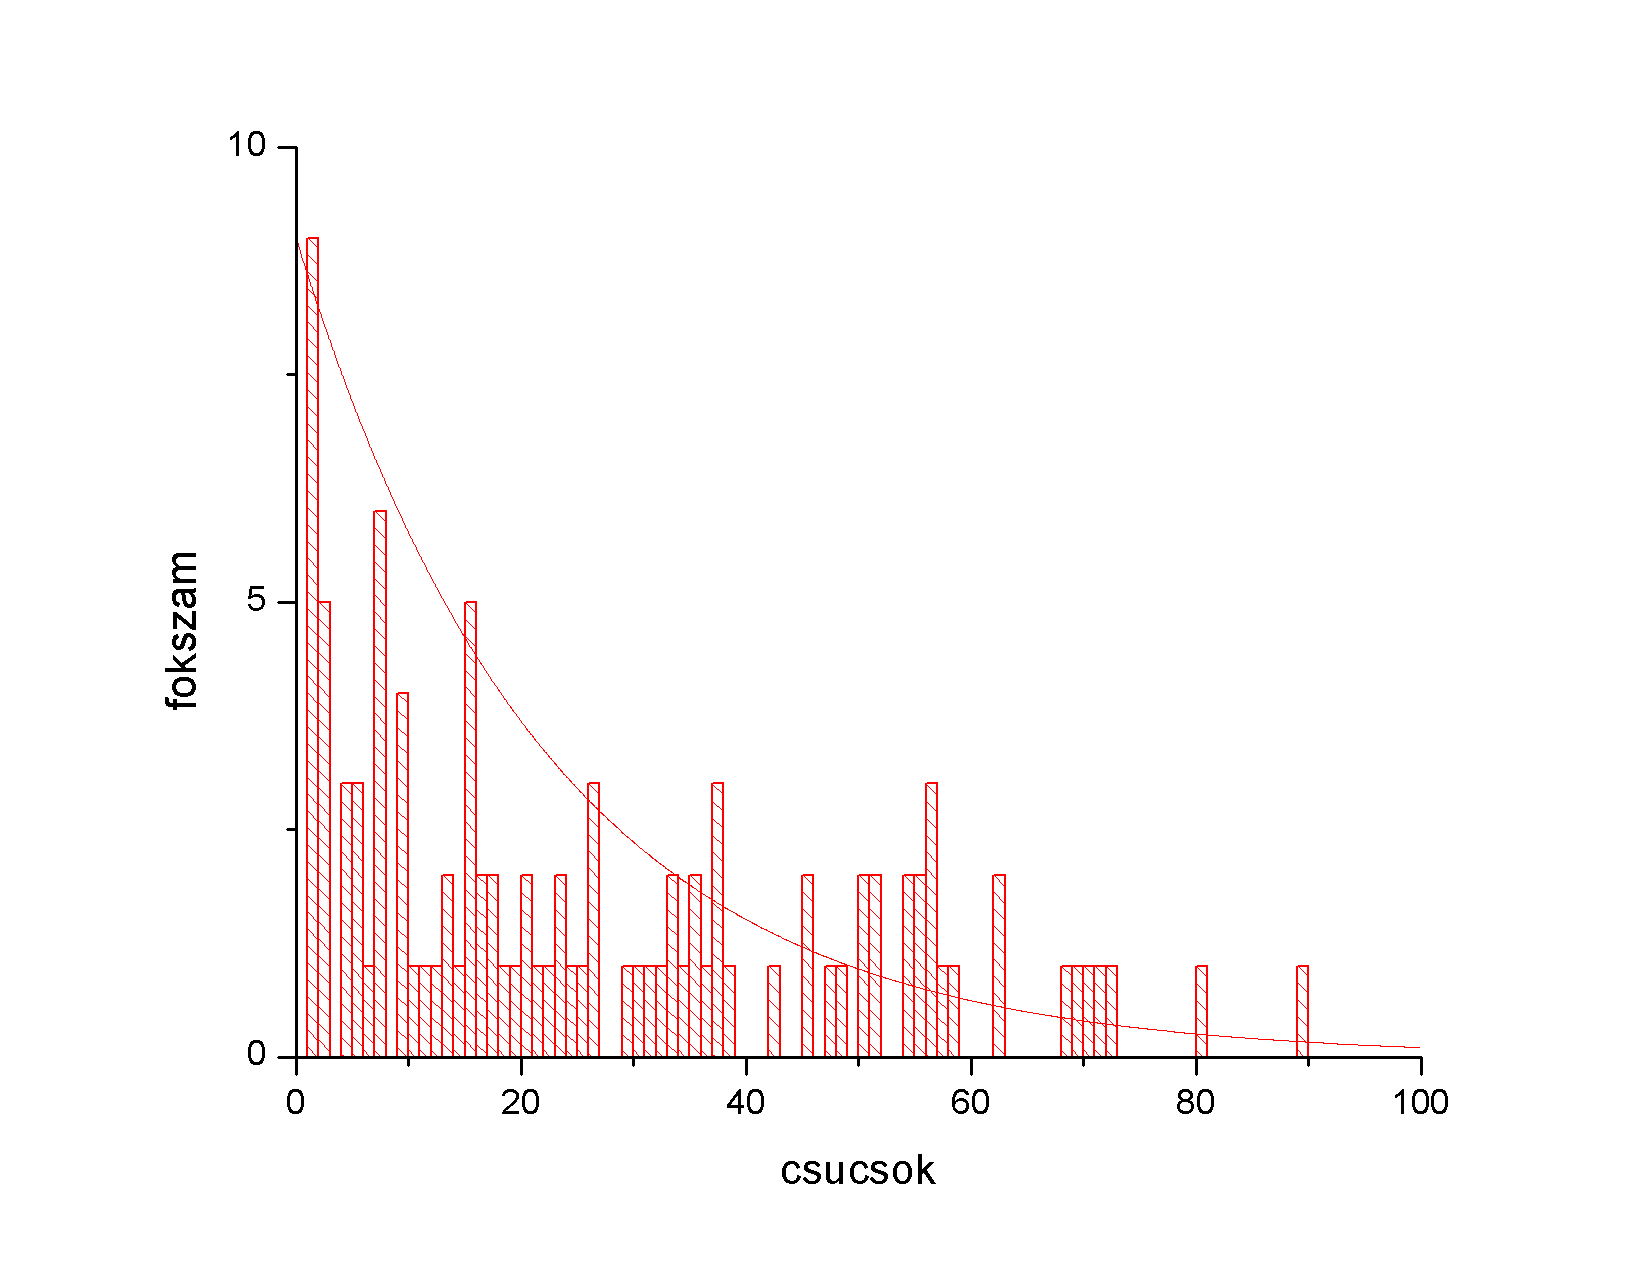
\includegraphics[width=\textwidth]{rekurzivfa}

\subsection{Eloszlás függvény hibája}
A kezdetben használt 100-as csúcs számú szimulációnak a standard hibája $\sim 1.4 \%$. Megvizsgáltam más csúcs számokra is. Azt találtam, hogy 50 csúcs esetén a $P_k$ standard hibája  $\sim 4.9 \%$





\subsection{Átlagos fokszám}



Az elméletből:
\begin{align}
&<k>=\sum_{k=0}^\infty kP_k=\sum_{k=0}^\infty k\frac{N_k}{N}=\frac{1}{N}\sum_{k=0}^\infty kN_k=\frac{2L}{N}\\
&<k>=\underline{1}
\end{align}
A szimulációból 100 csúcs esetén:
\begin{align}
&<k>=\underline{1.99}
\end{align}






\newpage


\section{Anti-preferenciális csatolás}
100 csomópontra a következő fokszámeloszlást kaptam:
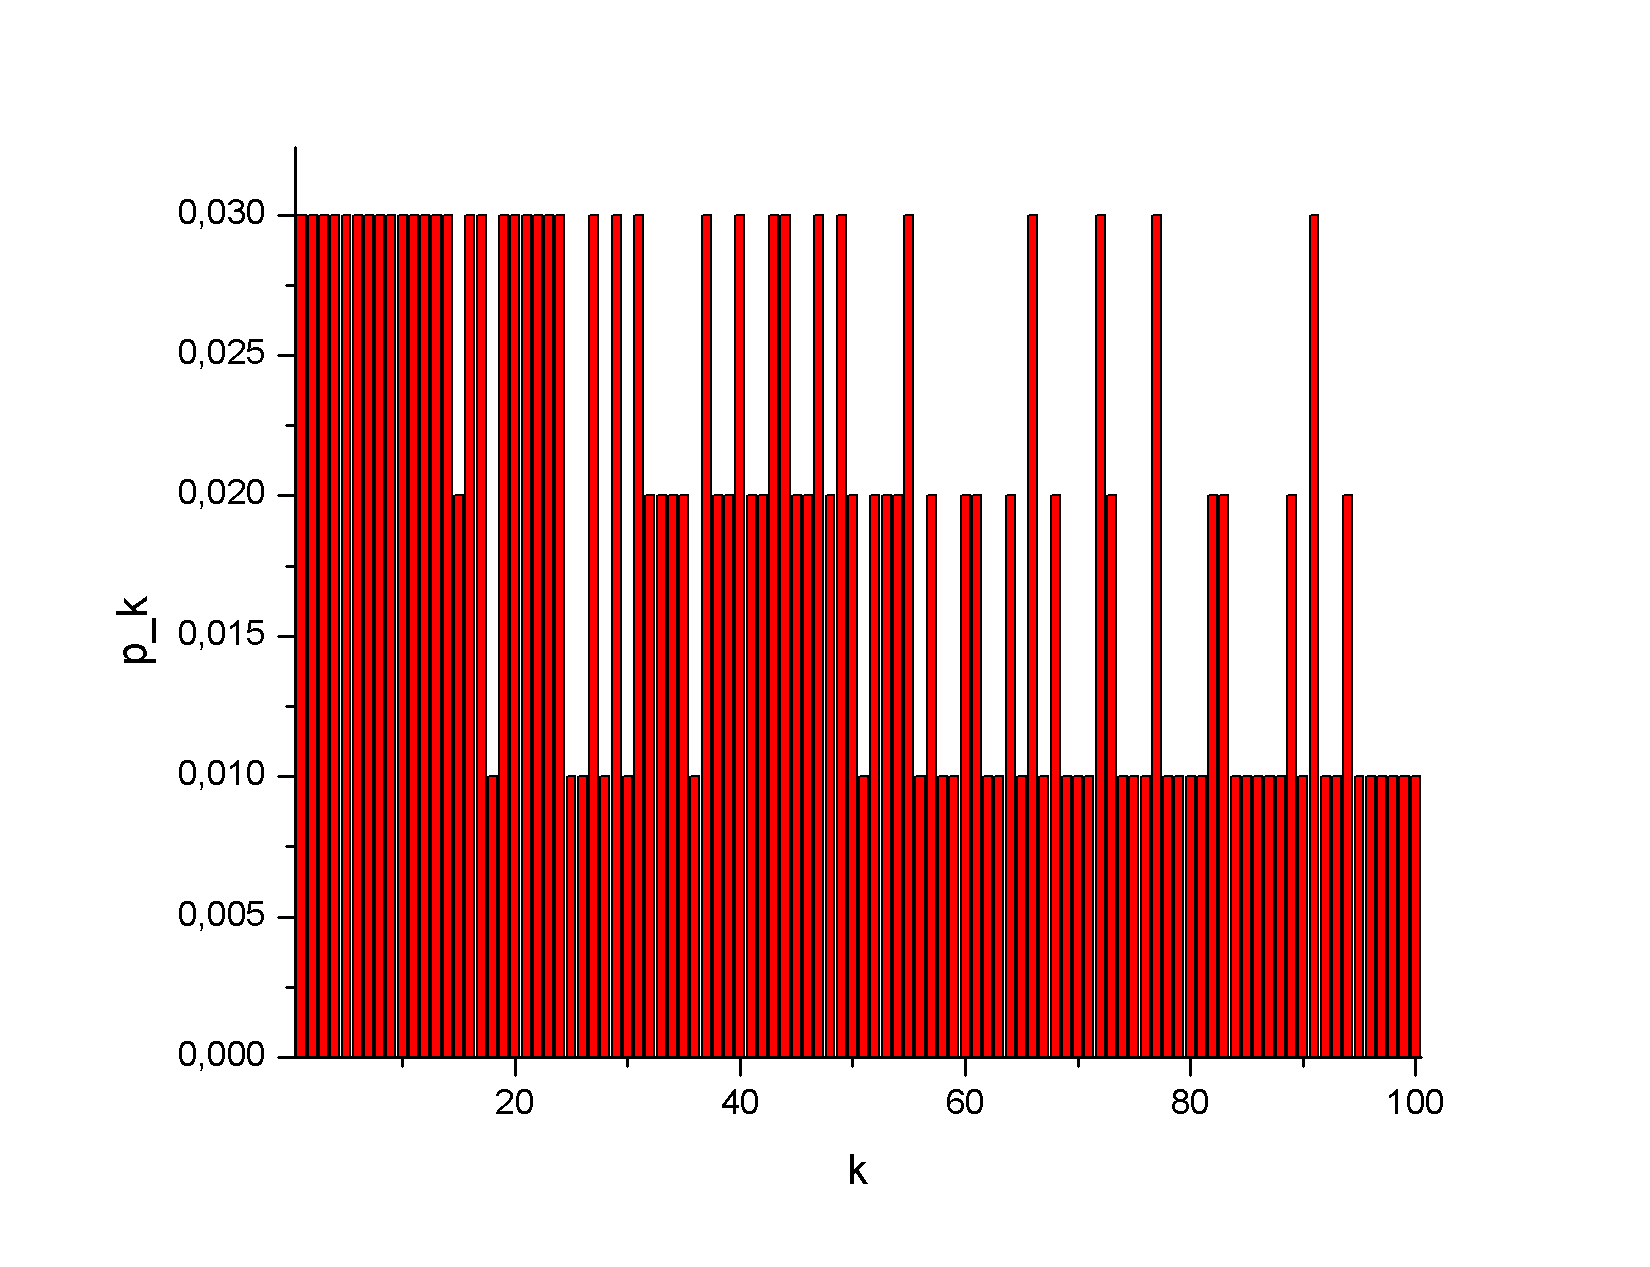
\includegraphics[width=\textwidth]{antipk}
Megfigyelhető, hogy a rekurzívhoz képest ez "simább" és kevésbé exponenciálisan lecsengő, ez megfelel a várakozásoknak, hiszen a kezdetek óta jelen lévő csúcsok ezzel a megkötéssel amit itt alkalmazunk nem tudnak felhalmozni nagy mennyiségű élet, úgy ahogyan azt a rekurzív fa esetében tették.
\subsection{Fokszám eloszlás}


\subsection{Nagy értékű k aszimptotikája}
Megvizsgáltam 1000 csomópontra is a fokszámeloszlást.

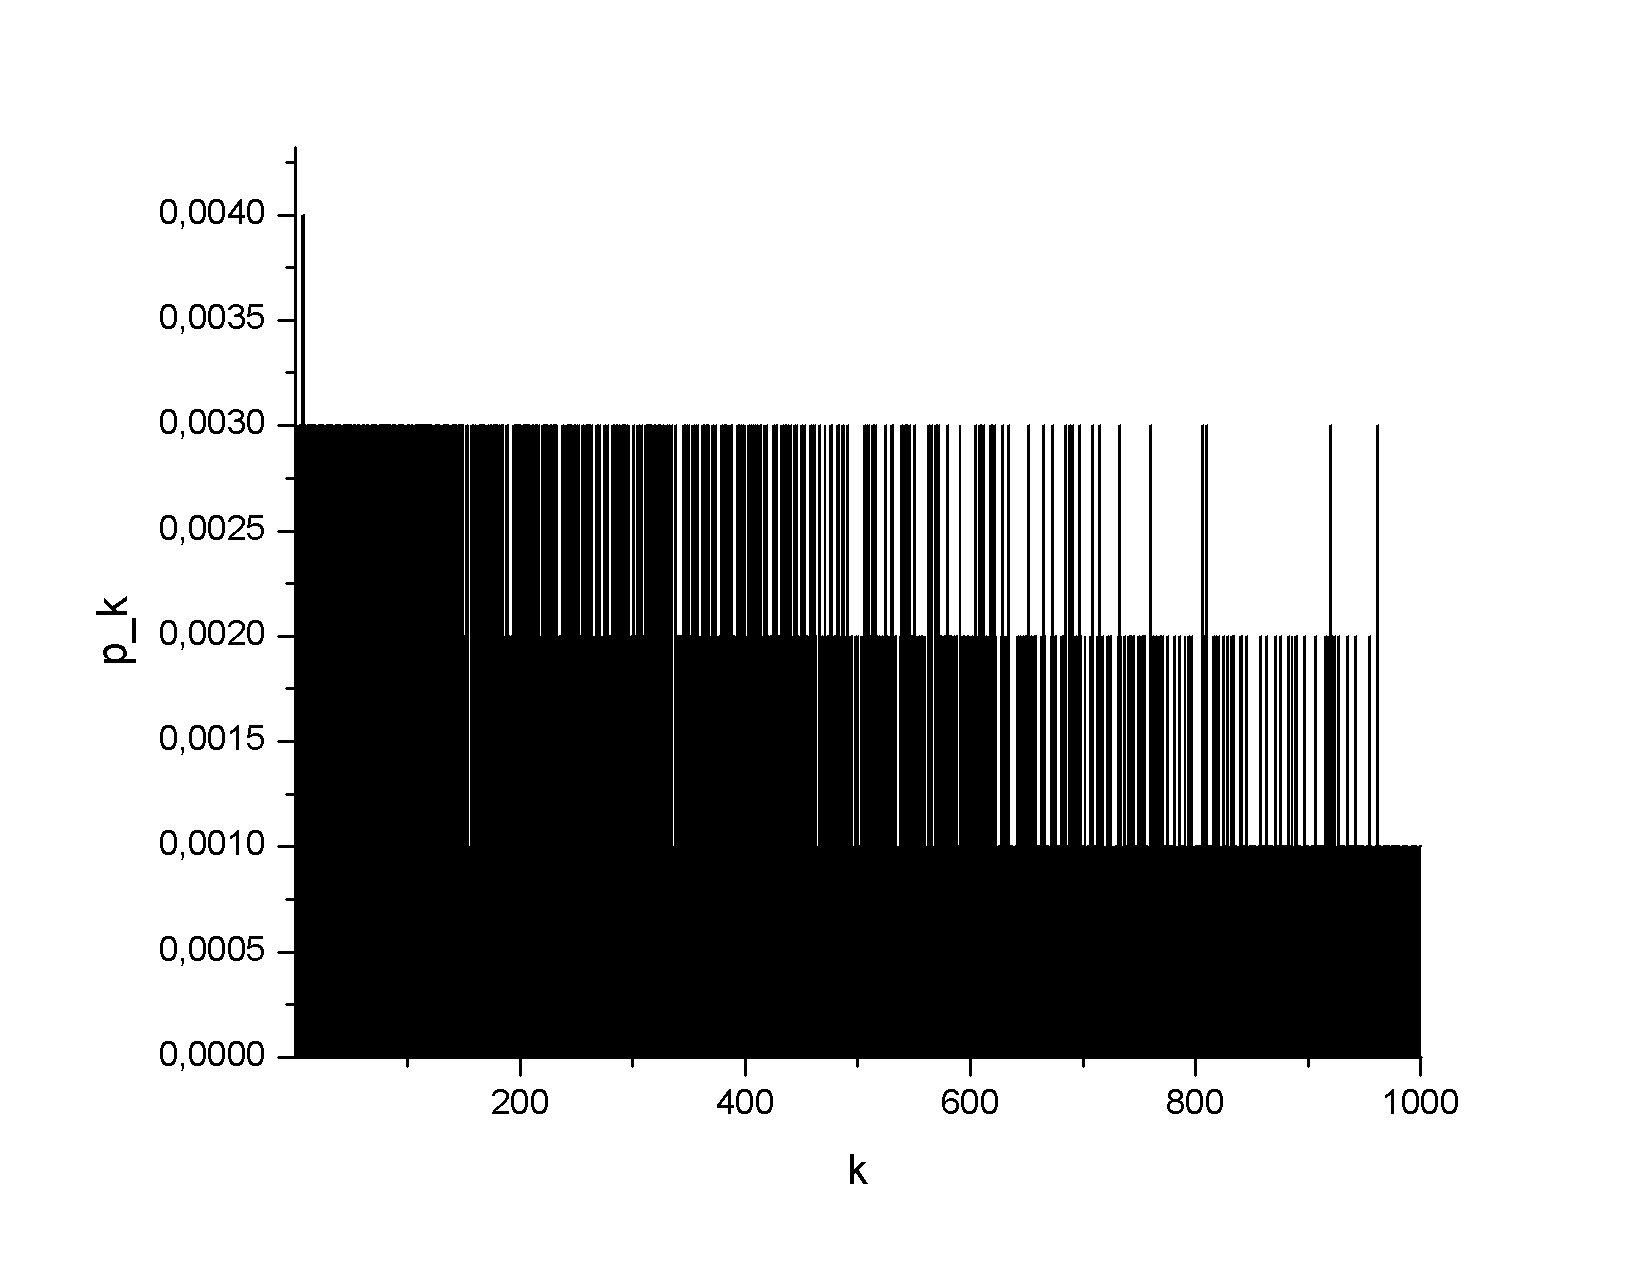
\includegraphics[width=\textwidth]{antipk1000}



\newpage

\section{Eltolt lineáris preferencia}



\begin{align}
P_k=&\frac{(k-1)+\lambda}{k+2+2\lambda}P_{k-1}=\frac{(k-1+\lambda)(k-2+\lambda)}{(k+2+2\lambda)(k+1+2\lambda)}P_k-2=\\
&\frac{(k-1+\lambda)(k-2+\lambda).....(1+\lambda)}{(k+2+2\lambda)(k+1+2\lambda)...(4+2\lambda)}P_1\\
\end{align}

\begin{align}
&\lambda=1\\
&P_k=\frac{k(k-1)...*2}{(k+4)(k+3)...*6}\frac{3}{5}=\frac{k!}{(k+4)!}*a=\frac{a}{(k+4)(k+3)(k+2)(k+1)}\approx \frac{1}{k^4} \approx \frac{1}{k^{3+\lambda}}
\end{align}


































\end{document}